\section{La realidad, <<The Electronic WasteLand>>}

Tal y como se ha visto a lo largo del artículo, los gobiernos aparentemente estan legislando para resolver el problema de la e-basuara aunque ya se ha visto que la legislación es muy laxa, debido a los altos costes de los procedimientos de reciclaje y de reutilización y los grandes lobbys de compañías fabricantes que no quieren incurrir en los mismos. Iniciativas para crear estandares que faciliten este proceso también se han iniciado pero todavía no han concretado en nada realmente útil y provechoso.

Al amparo de todo esto, han surgido un gran número de compañías, cuyo negocio es el reciclaje de la e-basura, atraidos por los impuestos y subvenciones que los gobiernos han establecido para la realización de estos servicios. 

Están también surgiendo empresas de innovación tecnológica que estan tratando de industrializar y simplificar el proceso para realizarlo más eficientemente y de forma más económica.

Sin embargo, todo esto, queda en un conjunto de buenos deseos y buenas intenciones. Las estadisticas oficiales muestran que solo un 33\% de la e-basura pasa por las plantas de reciclado y tal y como se ha podido ver en varios reportajes de investigación, como el reportaje de la cadena CBS News, <<The Electronic WasteLand>>, \cite{wasteland}, la realidad detras de estas empresas de reciclaje no siempre es lo que esperamos.

En este reportaje se muestra una compañía especializada en reciclaje de e-basura a la que ciudadanos de los Estados Unidos entregan sus viejos dispositivos pensando que van a ser reciclados. De hecho existen grandes colas de espera para poder entregar los dispositivos.

\begin{figure}[H]
\begin{center}
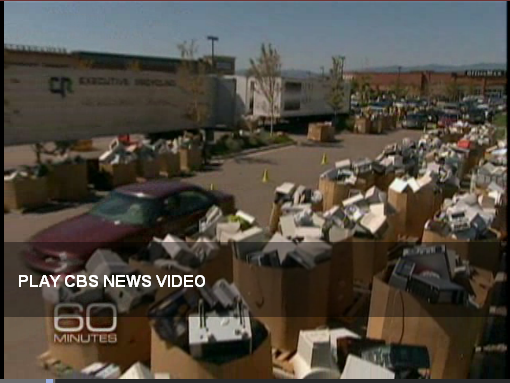
\includegraphics[width=0.5\textwidth]{img/screen1}
\caption{Screenshot reportaje CBS News - The Electronic WasteLand}
\end{center}
\end{figure}